\chapter{Dasar Teori}
\label{chap:dasar_teori}

Bab ini menjelaskan mengenai teori-teori yang digunakan dalam penelitian ini, antara lain penjelasan mengenai \textit{captive portal}, \textit{.NET framework}, \textit{Common Laguage Infrastructure}, \textit{Universal Windows Platform}, kelas WebView, dan kelas PasswordVault.



\section{\textit{Captive Portal}}
\label{sec:captive_portal}

\textit{Captive portal} adalah \textit{router}\footnote{Berdasarkan kamus bahasa inggris oxford, \textit{router} adalah alat yang meneruskan paket data ke bagian dari jaringan yang dituju.} atau \textit{gateway}\footnote{Berdasarkan kamus bahasa inggris oxford, gateway adalah alat yang digunakan untuk menghubungkan dua jaringan yang berbeda, biasanya berupa hubungan ke internet.} yang akan menutup koneksi eksternal sampai klien yang bersangkutan sudah terotentikasi\cite{Potter:2002}. Cara kerja \textit{captive portal} secara umum adalah sebagai berikut:

\begin{enumerate}
    \item{Memberikan alamat IP melalui DHCP pada perangkat yang baru terhubung.}
    \item{Tutup seluruh akses kecuali ke \textit{captive portal server}.}
    \item{Arahkan seluruh \textit{request} HTTP ke \textit{captive portal}.}
    \item{Tampilkan aturan penggunaan, informasi pembayaran, dan\/atau halaman \textit{login}.}
    \item{Jika pengguna telah menyetujui aturan penggunaan atau telah melakukan \textit{login}, buka akses.}
    \item{Opsional: Saat pengguna telah melewati batas waktu tertentu, tutup akses.}
\end{enumerate}

Akan tetapi, pada prakteknya, implementasi \textit{captive portal} sangat beragam dan bersifat \textit{ad-hoc}\cite{HTTPWG_CP:2016}. Beberapa perilaku \textit{captive portal} lain yang teramati adalah sebagai berikut:

\begin{itemize}
    \item{Memaksa pengguna untuk tetap membuka satu \textit{browser window}. Teknik ini membantu mencegah pencurian koneksi pengguna dengan duplikasi alamat MAC.}
    \item{Menggunakan otorisasi yang terbatas oleh waktu. Pengguna harus berinteraksi kembali dengan portal setelah waktu tertentu.}
\end{itemize}

\subsubsection{Kode Status HTTP 511}
\label{par:http_511}

Kode status HTTP adalah bilangan bulat positif yang terdiri dari 3 digit\cite{IETF_HTTP:2016}. Kode status ini dikirimkan sebagai hasil dari usaha untuk memahami \textit{request}. Kode status HTTP bersifat \textit{extensible}. Secara garis besar, kode status HTTP dibagi menjadi 5 bagian, yaitu:

\begin{itemize}
    \item{1xx (Informatif): \textit{Request} telah diterima dan proses dapat dilanjutkan.}
    \item{2xx (Berhasil): \textit{Request} telah diterima dan dimengerti.}
    \item{3xx (\textit{Redirection}): Aksi selanjutnya perlu dilakukan untuk memenuhi \textit{request}.}
    \item{4xx (Kesalahan Klien): \textit{Request} mengandung sintaks yang buruk.}
    \item{5xx (Kesalahan \textit{Server}): \textit{Server} tidak dapat memenuhi \textit{request} yang valid.}
\end{itemize}

Kode status HTTP 511 menandakan bahwa klien perlu melakukan otentikasi untuk mendapatkan akses pada jaringan yang bersangkutan\cite{IETF_HTTP_AdditionalStatus:2016}. Respon dengan kode status ini harus menyertakan \textit{link} ke sumber yang memungkinkan pengguna untuk memasukkan kredensial. Selain itu, respon dengan kode status ini tidak boleh diberikan oleh server tujuan. Respon ini dimaksudkan sebagai kontrol akses pada jaringan yang akan diberikan oleh komponen perantara dalam jaringan. Respon dengan kode status 511 tidak boleh disimpan oleh \textit{cache}.

\subsubsection{Kode Status HTTP 511 dan \textit{Captive Portal}}
\label{par:http_511_and_captive_portal}

Kode status 511 diciptakan untuk mengurangi masalah yang ditimbulkan oleh \textit{captive portal} kepada perangkat lunak yang mengharapkan respon dari server tujuan, bukan dari komponen perantara dalam jaringan. Sebagai contoh, perangkat lunak yang bersangkutan mengirimkan \textit{request} HTTP pada port TCP 80 sebagai berikut:

\begin{lstlisting}
GET /index.htm HTTP/1.1
Host: www.example.com
\end{lstlisting}

Saat menerima \textit{request} tersebut, server login akan mengirimkan respon dengan kode status 511:

\begin{lstlisting}
HTTP/1.1 511 Network Authentication Required
Content-Type: text/html

<html>
    <head>
        <title>Network Authentication Required</title>
        <meta http-equiv="refresh"
            content="0; url=https://login.example.net/">
    </head>
    <body>
        <p>You need to <a href="https://login.example.net/">
        authenticate with the local network</a> in order to gain
        access.</p>
    </body>
</html>
\end{lstlisting}

Respon ini memungkinkan klien untuk mendeteksi bahwa respon tersebut bukan berasal dari server tujuan. Selain itu, elemen meta pada HTML yang disajikan memungkinkan klien untuk melakukan login pada \textit{link} yang diberikan.



\section{\textit{.NET Framework}}
\label{sec:net_framework}

.NET adalah platform yang bersifat \textit{general purpose} untuk membangun aplikasi\cite{NET_PRIMER:2016}. .NET memberikan lingkungan untuk melakukan pemrograman \textit{high-level} dan tetap memberikan akses \textit{low-level} ke memori dan beberapa API. .NET memiliki beberapa implementasi berdasarkan standar \textit{open} .NET yang mendefinisikan dasar-dasar yang harus dimiliki oleh platform ini. Implementasi-implementasi ini memberikan dukungan bagi beberapa \textit{chip} (seperti x86/x64 dan ARM) dan beberapa sistem operasi (seperti Windows, Linux, iOS, Android, dan macOS).



\section{\textit{Common Language Infrastructure} (CLI)}
\label{sec:cli}

.NET memberikan kebebasan kepada \textit{developer} untuk memilih bahasa yang ingin digunakan. Hal ini dapat dilakukan selama bahasa tersebut mendukung .NET. Kebebasan memilih bahasa ini dimungkinkan karena .NET menggunakan spesifikasi \textit{Common Language Inrastructure} (CLI).

\begin{figure}[h]
    \centering
    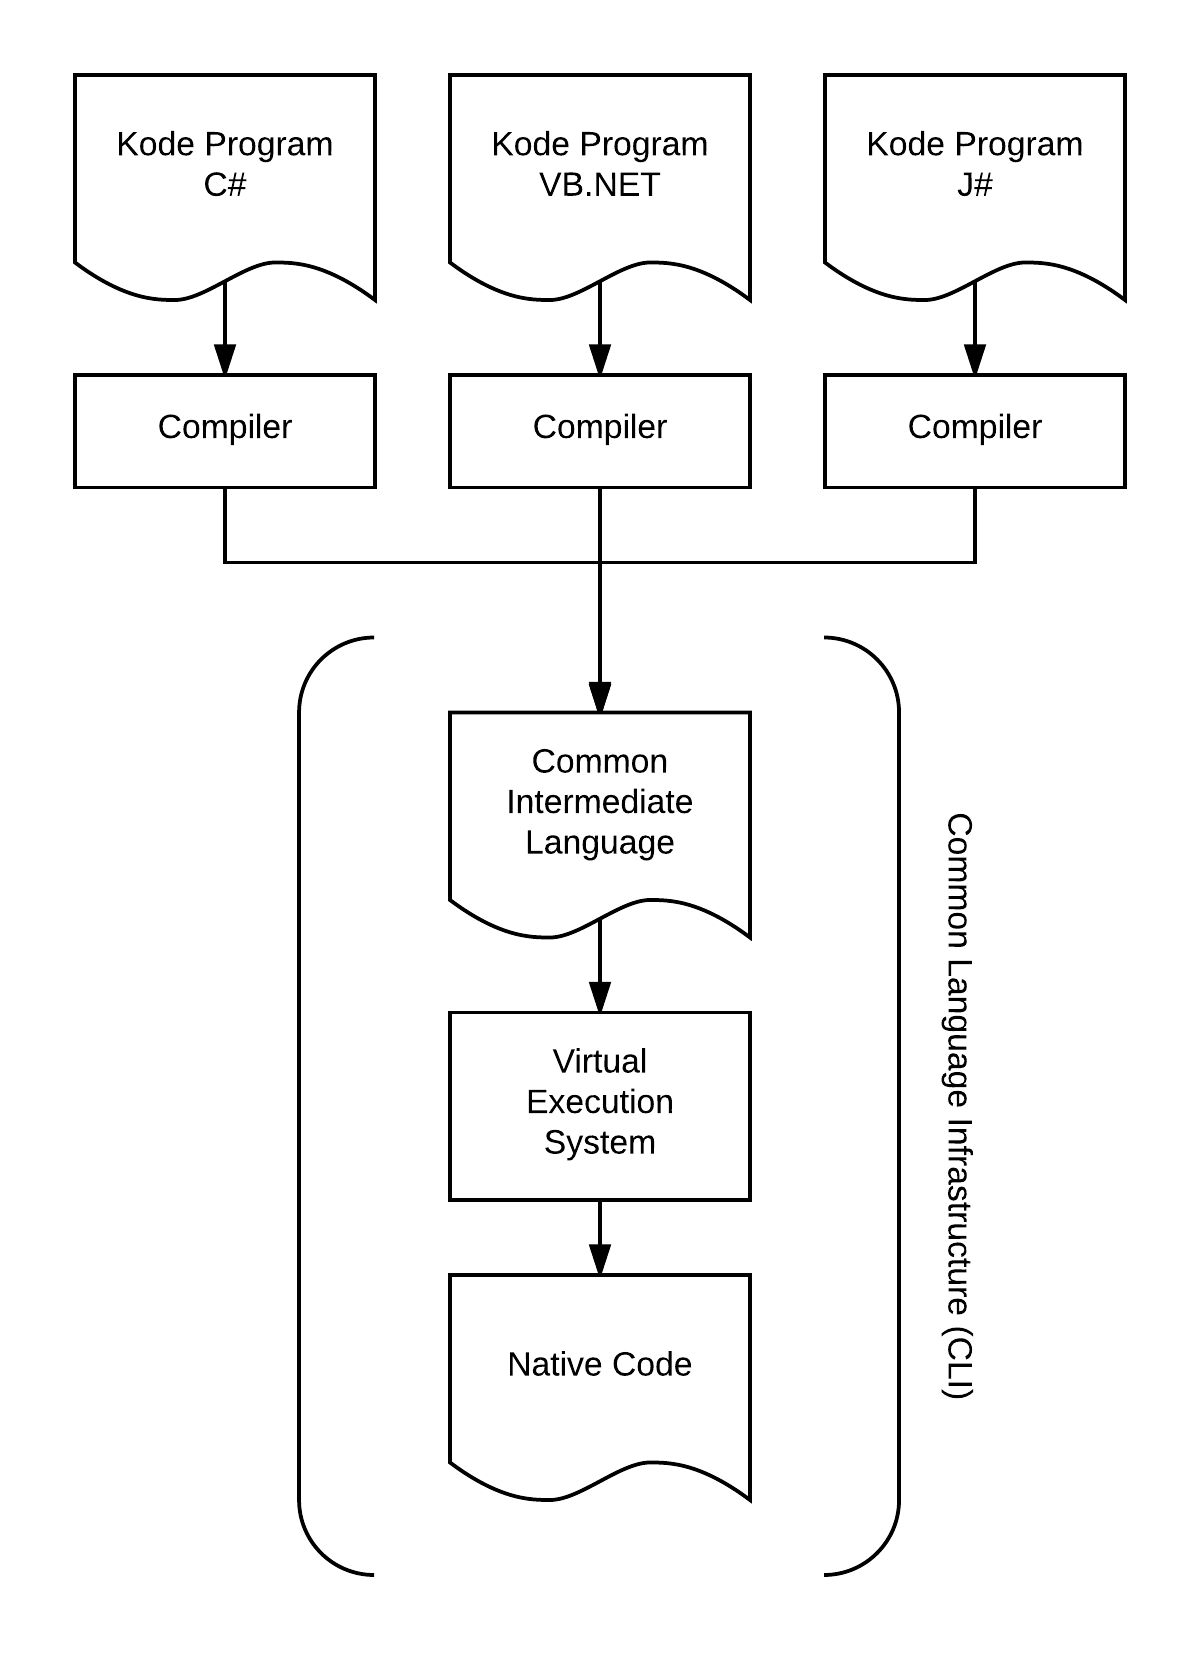
\includegraphics[scale=0.2]{Gambar/CLI.png}
    \caption[Diagram alir proses yang dilalui oleh kode program dalam CLI.]{Diagram alir proses yang dilalui oleh kode program dalam CLI.} 
    \label{fig:cli}
\end{figure}

Komponen-komponen penting dalam CLI di antaranya adalah\cite{CLI:2016}:

\begin{itemize}
    \item{\textit{Common Type System} (CTS)\\CTS memberikan \textit{type system} yang kaya dan mendukung tipe dan operasi yang ditemukan pada banyak bahasa pemrograman.}
    \item{\textit{Metadata}\\CLI menggunakan \textit{metadata} untuk menjelaskan dan mereferensi tipe-tipe yang didefinisikan oleh CTS.}
    \item{\textit{Common Language Spesification} (CLS)\\CLS adalah perjanjian desainer bahasa pemrograman dan desainer \textit{framework}. Perjanjian ini menentukan bagian minimal dari CTS yang harus diimplementasikan oleh bahasa pemrograman dan \textit{framework} yang bersangkutan.}
    \item{\textit{Virtual Execution System} (VES)\\VES mengimplementasikan model CTS dan memastikan hal tersebut berjalan sebagaimana mestinya. VES berfungsi untuk menjalankan program yang ditulis untuk CLI.}
\end{itemize}

Seperti yang dijelaskan pada Gambar \ref{fig:cli}, beberapa bahasa pemrograman yang kompatibel dengan .NET adalah C\#, VB.NET, dan J\#\cite{NET_PRIMER:2016}. Setelah kode program dari bahasa-bahasa tersebut diterjemahkan oleh \textit{compiler}nya masing-masing, maka akan terbentuk \textit{Common Intermediate Language} (CIL) yang kemudian akan dibaca dan dieksekusi oleh VES\cite{CLI:2016}. Implementasi VES pada .NET bernama \textit{Common Language Runtime} (CLR).



\section{\textit{Universal Windows Platform} (UWP)}
\label{sec:uwp}

Windows 8 memperkenalkan \textit{Windows Runtime} (WinRT) yang merupakan arsitektur aplikasi umum untuk Windows\cite{UWP:2016}. Saat Windows Phone 8.1 keluar, Windows Runtime pada Windows 8 dan Windows Phone 8.1 disejajarkan agar \textit{developer} dapat membangun satu aplikasi yang dapat dijalankan pada Windows 8 dan Windows Phone 8.1. \textit{Universal Windows Platform} (UWP) pertama kali diperkenalkan pada Windows 10 sebagai perubahan dari model \textit{Windows Runtime}. UWP tidak hanya dapat memanggil API dari WinRT, namun juga API spesifik dari device yang bersangkutan (seperti Win32 dan .NET).



\section{Kelas WebView Pada UWP}
\label{sec:webview}

Kelas WebView pada UWP memungkinkan \textit{developer} untuk menampung konten HTML pada suatu aplikasi\cite{WinAPI:2016}. WebView tidak mendukung masukkan pengguna seperti \textit{key-down}, \textit{key-up}, dan \textit{pointer-pressed}. Oleh karena itu, dibutuhkan metode lain yang melibatkan InvokeScriptAsync dengan fungsi \textit{eval} javascript untuk menggunakan HTML \textit{event handler} dan fungsi window.external.notify untuk menangani event dari HTML pada aplikasi.

Beberapa \textit{property} yang dimiliki oleh WebView adalah:

\begin{itemize}
    \item{DocumentTitle\\Menyimpan \textit{title} dari dokumen yang sedang ditampilkan dalam bentuk String.}
    \item{BaseUri\\Menyimpan \textit{uri} dari dokumen yang sedang ditampilkan dalam bentuk Uri.}
\end{itemize}

Beberapa \textit{method} yang dimiliki oleh WebView adalah:

\begin{itemize}
    \item{InvokeScriptAsync(String scriptName, String[] arguments)\\Method ini digunakan untuk melakukan eksekusi script tertentu pada HTML dengan argumen yang diberikan dalam bentuk \textit{array of string}.}
    \item{Navigate(Uri source)\\Method ini digunakan untuk membuka URI\footnote{URI adalah singkatan dari Uniform Resource Identifier.} tertentu.}
\end{itemize}

Salah satu \textit{event} yang dimiliki oleh kelas WebView adalah \textit{event} ScriptNotify. \textit{Event} ini berguna untuk menangkap hasil dari fungsi javascript window.external.notify.



\section{Kelas PasswordVault Pada Windows}
\label{sec:passwordvault}

Kelas PasswordVault merupakan komponen dari Windows Runtime API, dan bukan .NET\cite{WinAPI:2016}. Kelas ini merepresentasikan pengunci kredensial. Kredensial yang disimpan menggunakan kelas ini hanya dapat diakses oleh aplikasi atau \textit{service} yang bersangkutan. Beberapa \textit{method} yang dimiliki oleh kelas PasswordVault adalah:

\begin{itemize}
    \item{Add(PasswordCredential credential)\\\textit{Method} ini berfungsi untuk memasukkan kredensial.}
    \item{Retrieve(String resource, String userName)\\\textit{Method} ini berfungsi untuk mengambil kredensial yang tersimpan di dalam objek PasswordVault.}
    \item{Remove(PasswordCredential credential)\\\textit{Method} ini berfungsi untuk menghapus kredensial yang tersimpan di dalam objek PasswordVault.}
\end{itemize}

